%% Electronic phenotyping as coarsening at random:
%% identifiability of clinical states from diagnosis codes.
%% Conference-format draft (target: 12 pages incl. references).

\documentclass[11pt,letterpaper]{article}

%% ============================================================================
%% Packages
%% ============================================================================

\usepackage{amsmath,amsthm,amssymb}
\usepackage{mathtools}
\usepackage{bm}
\usepackage{graphicx}
\graphicspath{{figures/}}
\usepackage{float}
\usepackage{booktabs}
\usepackage[shortlabels]{enumitem}
\usepackage[margin=1in]{geometry}
\usepackage{microtype}
\usepackage[colorlinks=true,linkcolor=blue,citecolor=blue,urlcolor=blue]{hyperref}
\usepackage{natbib}
\usepackage{cleveref}

%% Theorem environments
\theoremstyle{plain}
\newtheorem{theorem}{Theorem}
\newtheorem{proposition}[theorem]{Proposition}
\newtheorem{lemma}[theorem]{Lemma}
\newtheorem{corollary}[theorem]{Corollary}

\theoremstyle{definition}
\newtheorem{definition}[theorem]{Definition}
\newtheorem{condition}{Condition}
\crefname{condition}{Condition}{Conditions}
\Crefname{condition}{Condition}{Conditions}

\theoremstyle{remark}
\newtheorem{remark}[theorem]{Remark}

%% Macros
\newcommand{\E}{\mathbb{E}}
\newcommand{\Prob}{\mathbb{P}}
\newcommand{\R}{\mathbb{R}}
\newcommand{\1}{\mathbf{1}}
\newcommand{\X}{X}
\newcommand{\Y}{Y}

%% Title
\title{Electronic phenotyping as coarsening at random:\\
       identifiability of clinical states from diagnosis codes}

\author{
  Alexander Towell \\
  Department of Computer Science \\
  Southern Illinois University Edwardsville \\
  \texttt{lex@metafunctor.com} \\
  ORCID: \href{https://orcid.org/0000-0001-6443-9897}{0000-0001-6443-9897}
}

\date{\today}

\begin{document}

\maketitle

\begin{abstract}
\noindent\textbf{Objective:} To formalize identifiability conditions
for electronic phenotyping when diagnosis codes are informative of
latent clinical severity, and to characterize the bias of code-only
and chart-review-calibrated prevalence estimators.

\noindent\textbf{Materials and Methods:} We embed code-based
phenotyping in the coarsening-at-random framework: the true clinical
state is the latent cause, the observed diagnosis code set is the
candidate set, the coding process is the masking mechanism, and a
chart-reviewed patient is a singleton candidate set. We identify
informative coding (sicker patients are coded more) as the failure of
the non-informative-masking condition C2, and we analyze identifiability
and bias under this failure.

\noindent\textbf{Results:} A glass-ceiling theorem shows that
(prevalence, code sensitivity, code specificity) is jointly
non-identifiable from code data alone. An identifiability theorem
shows that a chart-reviewed subsample covering both classes identifies
the coding model and yields the Rogan-Gladen plug-in estimator. A
code-frequency consistency theorem shows the fitted model reproduces
the empirical code frequency exactly at any interior MLE, so
marginal-fit diagnostics are blind to prevalence bias. A bias bound
shows the code-only bias is controlled by the severity-coding
correlation and the calibrated estimator's residual bias by the
case-mix gap. Simulation confirms all four results; the bias sign can
flip from negative to positive depending on whether sensitivity
deficit or false-positive inflation dominates.

\noindent\textbf{Discussion:} The glass ceiling is the EHR-coding
instance of the partial-identification results for misclassified data
\citep{horowitz1995identification,molinari2008partial}, and the
chart-review estimator coincides with the calibrated EHR prevalence
estimators of \citet{tong2020augmented} and
\citet{beesley2022samba}. The framework's contribution is positioning:
it names the failing assumption (C2) and quantifies the bias, placing
Hui-Walter latent class models, Rogan-Gladen correction, and
verification-bias correction in one coarsening vocabulary.

\noindent\textbf{Conclusion:} Chart review is a necessity, not a
luxury; its identifying value is bounded by case-mix representativeness.
\end{abstract}

\section{Introduction}
\label{sec:intro}

Electronic health records (EHRs) generate administrative data on every
patient encounter: International Classification of Diseases (ICD)
diagnosis codes, procedure codes, and medication orders. A large
secondary-use literature reuses this data to answer the question
\emph{does a patient have clinical condition $Z$?} This task is
\emph{electronic phenotyping}: inferring a latent clinical state from
coarse administrative signals \citep{banda2018phenotyping,
hripcsak2013correlating}. Phenome-wide association studies
\citep{denny2010phewas}, the Electronic Medical Records and Genomics
network \citep{gottesman2013emerge,newton2013validation}, the PheKB
algorithm catalog \citep{kirby2016phekb}, anchor-and-learn classifiers
\citep{halpern2016anchor}, high-throughput phenotyping
\citep{liao2015highthroughput}, semi-supervised methods such as
PheNorm \citep{yu2018phenorm} and PheCAP \citep{zhang2019phecap}, and
probabilistic phenotypes \citep{pivovarov2015learning} all build
phenotype definitions on top of diagnosis codes and related EHR
features.

The difficulty is that the diagnosis code is a noisy and
\emph{systematically biased} proxy for the true clinical state. A code
is generated only when a clinician records an encounter, when a billing
process attaches a code to that encounter, and when coverage and
reimbursement incentives make that code worth recording. The fraction
of patients carrying a code for condition $Z$ is therefore not the
prevalence of $Z$. Code sensitivity (the probability that a true case
is coded) and code specificity (the probability that a non-case is not
coded) are both unknown, and both depend on factors, encounter
frequency, disease severity, and local coding practice, that have
nothing to do with the underlying epidemiology
\citep{hripcsak2013correlating,carrell2014surveillance}.

\subsection{The bridge to masked-data inference}

The central observation of this paper is that electronic phenotyping
is mathematically isomorphic to the masked-data series-system
identifiability problem of \citet{towell2026masked}. In that
framework, a latent cause is masked, but a \emph{candidate set}
containing it is observed; coarsening-at-random conditions
\citep{heitjan1991ignorability,gill1997coarsening} on the masking
mechanism determine whether the cause-level parameters can be
recovered.

The translation to phenotyping is direct. The true clinical state
$\Y \in \{0,1\}$ is the latent cause. The set of clinical states
consistent with a patient's observed diagnosis codes is the candidate
set. The coding process, $\Prob(\text{code} \mid \Y)$, shaped by
clinician behavior and billing, is the masking mechanism. A
chart-reviewed (clinician-adjudicated) patient, for whom the true
state is established by manual record review, is a singleton candidate
set: the truth is known exactly. The C1-C2-C3 conditions for ignorable
coarsening port directly. This framework has been applied to scRNA-seq
zero inflation \citep{towell2026scrnacoarsening} and to spatial
transcriptomics deconvolution \citep{towell2026spatialcoarsening};
electronic phenotyping is the present application.

The phenotyping case has a distinctive feature. In the transcriptomics
applications the coarsening mechanism is approximately non-informative
once technical covariates are modeled. In phenotyping it is
\emph{structurally} informative. Sicker patients have more encounters
and are coded more; billing incentives change which codes are recorded;
surveillance and detection intensity track disease severity
\citep{haut2011surveillance}. The coarsening-at-random condition that
fails is C2, non-informative coding. This single observation explains
why code-only prevalence estimates are biased and why chart review is
a necessity rather than a luxury.

\subsection{Prior work on latent-class phenotyping}

Estimating disease status without a gold standard has a deep prior
literature that we do not claim to originate.
\citet{rogan1978estimating} gave the canonical
sensitivity-and-specificity correction for apparent prevalence, the
plug-in estimator that recovers $\pi$ from the observed code
frequency once $\mathrm{sens}$ and $\mathrm{spec}$ are known; this
paper's chart-review estimator is that estimator with the two error
rates supplied by the adjudicated subsample. \citet{hui1980estimating}
introduced the latent-class model for estimating diagnostic-test error
rates when no perfect reference test exists, and
\citet{dawid1979maximum} gave the EM algorithm for rater-error rates
that is the methodological ancestor of all such work. The
verification-bias literature (\citealp{begg1983assessment}; see
\citealp{hubbard2020outcome} for a recent phenotyping-specific
treatment) recognized that when verification of disease status is
selective, naive estimates of test accuracy and prevalence are biased;
the case-mix gap of \cref{cor:casemix} is the coarsening recasting of
this phenomenon. eMERGE
\citep{gottesman2013emerge} and PheKB \citep{kirby2016phekb} are
large-scale phenotyping efforts, and the anchor-and-learn framework
\citep{halpern2016anchor} uses high-precision signals in a way
structurally analogous to singleton candidate sets. Our contribution
is not latent-class phenotyping itself. It is the masked-cause
unification: a single coarsening vocabulary that classifies the
failure modes of code-based phenotyping through the C1-C2-C3
conditions, pinpoints informative coding as the C2 violation, and
quantifies the resulting bias.

\subsection{Contributions}

We contribute:

\begin{itemize}
\item \textbf{A bridge from electronic phenotyping to masked-data
  inference} (\cref{sec:translation}), with an explicit translation
  table mapping the coding mechanism to the masking mechanism and a
  chart-reviewed patient to a singleton candidate set.

\item \textbf{A glass-ceiling theorem} (\cref{thm:glass-ceiling},
  \cref{sec:identifiability}): with an unrestricted coding mechanism,
  prevalence, code sensitivity, and code specificity are jointly
  non-identifiable from code data alone. This formalizes why the
  fraction of patients carrying a code is a biased prevalence
  estimate.

\item \textbf{An identifiability theorem with chart review}
  (\cref{thm:identifiability-chart}, \cref{sec:identifiability}): a
  chart-reviewed subsample covering both diseased and non-diseased
  patients identifies the coding model, and cohort prevalence then
  becomes identifiable. This is the direct analog of the spike-in
  identifiability theorem of \citet{towell2026scrnacoarsening}.

\item \textbf{A code-frequency consistency theorem}
  (\cref{thm:code-total}, \cref{sec:identifiability}): a fitted
  phenotype model reproduces the marginal observed code frequencies
  exactly at an interior MLE. Marginal-fit checks therefore cannot
  detect prevalence bias.

\item \textbf{A bias bound under informative coding}
  (\cref{thm:bias-informative}, \cref{sec:methodology}): when code
  sensitivity correlates with latent disease severity, a C2 violation,
  the code-only prevalence estimator has bias bounded by a function of
  the severity-coding correlation. The chart-review-calibrated
  estimator's residual bias is bounded by the case-mix gap between the
  chart-reviewed subsample and the cohort, the analog of the
  ERCC-versus-endogenous capture-efficiency gap in
  \citet{towell2026scrnacoarsening}.

\item \textbf{Simulation validation} (\cref{sec:validation}), with a
  MIMIC-IV \citep{johnson2023mimiciv} real-data application described.
\end{itemize}

The paper's central message: code-based prevalence estimation is
biased by structure, not by accident, because coding is informative
and C2 fails. The bias is not directional in a simple way: depending
on the balance between code sensitivity and false-positive inflation,
code-only prevalence can understate the truth, overstate it, or pass
through zero as the severity-coding correlation varies (see
\cref{sec:validation}, \cref{tab:informative}). Chart review supplies
the singleton candidate sets that restore identifiability, and its
value is quantified by how well the reviewed subsample represents the
cohort.

\section{Masked-data inference: brief primer}
\label{sec:background}

We summarize the masked-data identifiability framework
\citep{towell2026masked,heitjan1991ignorability}. Readers familiar
with this work or with \citet{towell2026scrnacoarsening,
towell2026spatialcoarsening} can skim to \cref{sec:translation}.

Consider $m$ independent components in series. Each component $j$ has a
parametric distribution $f_j(\cdot;\theta_j)$ for its lifetime $T_{ij}$
in system $i$. The system fails at $T_i = \min_j T_{ij}$ with cause
$K_i = \arg\min_j T_{ij}$. We observe $T_i$ but not $K_i$ directly;
instead we observe a \emph{candidate set} $C_i \subseteq \{1,\ldots,m\}$
thought to contain the failed component.

The joint likelihood factorizes as
\begin{equation}
  f(t, k, c; \theta)
  = h_k(t; \theta_k) \prod_{\ell} R_\ell(t; \theta_\ell)
    \cdot \Prob_\theta\{C_i = c \mid T_i = t, K_i = k\},
  \label{eq:bg-joint}
\end{equation}
where $h_\ell$ is the component-$\ell$ hazard and $R_\ell$ its survival
function. The third factor is the unknown masking mechanism.

Three coarsening conditions allow the masking factor to drop from the
score:

\begin{condition}[Support, C1]
\label{cond:c1}
$\Prob\{K_i \in C_i\} = 1$.
\end{condition}

\begin{condition}[Symmetry, C2]
\label{cond:c2}
$\Prob_\theta\{C_i=c \mid T_i=t, K_i=j\} = \Prob_\theta\{C_i=c \mid
T_i=t, K_i=k\}$ for all $j,k \in c$.
\end{condition}

\begin{condition}[Parameter independence, C3]
\label{cond:c3}
$\Prob_\theta\{C_i=c \mid T_i, K_i\}$ does not depend on $\theta$.
\end{condition}

Under all three, the likelihood collapses to
\begin{equation}
  L_i(\theta) \propto \left[\prod_\ell R_\ell(t_i;\theta_\ell)\right]
  \cdot \left[\sum_{j \in c_i} h_j(t_i; \theta_j)\right].
  \label{eq:bg-c1c2c3}
\end{equation}

\citet[Theorem 8]{towell2026masked} establish identifiability:

\begin{theorem}[Identifiability under C1--C2--C3]
\label{thm:bg-id}
Under \cref{cond:c1,cond:c2,cond:c3} and standard regularity, full
column rank $m$ of the augmented candidate-set matrix $\tilde{C} \in
\{0,1\}^{n \times m}$ is \emph{sufficient} for $\theta$ to be
identifiable. Separability is necessary but not in general
sufficient (a separating mechanism can leave $\tilde{C}$
rank-deficient, e.g. $m=4$ with candidate sets
$\{1,2\},\{3,4\},\{1,3\},\{2,4\}$).
\end{theorem}

\emph{Singleton} candidate sets ($|c_i|=1$) are critical: each isolates
a single component contribution in \eqref{eq:bg-c1c2c3} and adds an
identifying row to $\tilde{C}$.

The condition that does the conceptual work in this paper is C2.
\Cref{cond:c2} requires the candidate set to be generated
symmetrically with respect to which masked cause is true. When the
masking mechanism depends on the latent cause in a way not captured by
the modeled structure, C2 fails, the masking factor no longer drops
from the score, and cause-level parameters become biased. This is the
\emph{informative coarsening} regime. The sensitivity of estimates to
C2 violations is studied directly in \citet{towell2026mdrelax}.

The framework has been ported to single-cell RNA sequencing zero
inflation \citep{towell2026scrnacoarsening} and to spatial
transcriptomics deconvolution \citep{towell2026spatialcoarsening}. We
now port it to electronic phenotyping. Two features distinguish the
phenotyping case. First, the latent cause is binary: a patient either
has condition $Z$ or does not. Second, and more important, the
coarsening mechanism is structurally informative. The coding process
depends on disease severity, encounter frequency, and billing
incentives, so C2 is not an approximation that holds after modeling
technical covariates; it is the condition that fails.

\section{Translation: electronic phenotyping as a coarsening problem}
\label{sec:translation}

\subsection{The data-generating process}

Consider a cohort of $n$ patients. Patient $i$ has a true clinical
state $\Y_i \in \{0,1\}$, where $\Y_i = 1$ indicates that the patient
has condition $Z$. The cohort prevalence is $\pi = \Prob(\Y_i = 1)$.

Each patient also has a latent severity $S_i$, a scalar summarizing how
advanced or symptomatic the condition is (for $\Y_i = 0$ patients, $S_i$
summarizes competing-condition burden or encounter intensity). Severity
is stochastically larger among true cases: $\E[S_i \mid \Y_i = 1] >
\E[S_i \mid \Y_i = 0]$.

The EHR records a diagnosis code for condition $Z$ through a coding
mechanism. Write $C_i \in \{0,1\}$ for the indicator that the code is
present. The coding mechanism is
\begin{equation}
  \Prob(C_i = 1 \mid \Y_i = 1, S_i)
    = \mathrm{logit}^{-1}(b_0 + b_1 S_i),
  \qquad
  \Prob(C_i = 1 \mid \Y_i = 0)
    = \mathrm{fpr},
  \label{eq:trans-coding}
\end{equation}
so that the code sensitivity for a true case rises with severity when
$b_1 > 0$, and code specificity is $1 - \mathrm{fpr}$. The marginal
code sensitivity is $\mathrm{sens} = \E[\,\mathrm{logit}^{-1}(b_0 + b_1
S) \mid \Y = 1\,]$. Additional coarse features, a procedure code or a
medication order, each carry their own sensitivity and specificity and
enter the same way.

The slope $b_1$ is the crux. When $b_1 = 0$, coding depends on $\Y$
only, not on severity, and the coarsening is non-informative: C2 holds.
When $b_1 > 0$, sicker true cases are preferentially coded; the
candidate set (the codes) carries information about the latent severity
beyond the latent state, and C2 fails. This is the
\emph{informative-coding} regime, and it is the realistic one: a true
case who is asymptomatic and never presents for care is rarely coded,
while a true case who is hospitalized is coded repeatedly.

The phenotyping problem is: given the observed codes $\{C_i\}$ for the
full cohort, and for a chart-reviewed subsample the adjudicated true
states $\{\Y_i\}$, recover the cohort prevalence $\pi$ and the coding
model.

\subsection{The translation}

\Cref{tab:translation} states the explicit correspondence to
masked-data inference.

\begin{table}[ht]
\centering
\small
\begin{tabular}{@{}p{0.40\linewidth} p{0.56\linewidth}@{}}
\toprule
\textbf{Masked-data framework} & \textbf{Electronic phenotyping} \\
\midrule
Component / latent cause
  & True clinical state / phenotype $\Y$ \\
Candidate set $c_i$
  & States consistent with the observed diagnosis codes \\
Masking probability
  & Coding mechanism $\Prob(\text{code} \mid \text{true state})$,
    shaped by clinician behavior and billing \\
Singleton candidate set $|c_i| = 1$
  & A chart-reviewed / clinician-adjudicated patient \\
C1 (truth in candidate set)
  & The true state is consistent with the codes;
    violated by gross miscoding \\
\textbf{C2} (coarsening at random): conditional on the candidate set, the masking distribution does not depend on which element is the true cause
  & Concretely: coding depends on $\Y$ only through modeled structure,
    not on prevalence or severity; \emph{violated} when coding
    intensity tracks severity (surveillance / detection bias) \\
C3 (parameter independence)
  & Coding-mechanism parameters distinct from prevalence;
    \emph{violated} when billing intensity tracks prevalence (a clinic
    facing a documented outbreak codes more aggressively, coupling
    sensitivity to the prevalence it is meant to estimate) \\
\bottomrule
\end{tabular}
\caption{Translation between the masked-data framework
\citep{towell2026masked} and electronic phenotyping. The C2 row is
load-bearing: informative coding is precisely the C2 violation.}
\label{tab:translation}
\end{table}

The phenotyping case is the binary specialization of the masked-cause
problem: the latent cause $\Y$ takes two values, and a patient with no
code at all has candidate set $\{0,1\}$ (the truth is unresolved),
while a chart-reviewed patient has a singleton candidate set
($\{0\}$ or $\{1\}$). The conceptual content is in the masking
mechanism. In the transcriptomics applications
\citep{towell2026scrnacoarsening,towell2026spatialcoarsening} the
coarsening mechanism is approximately non-informative once technical
covariates are modeled, so C2 holds and the difficulty is a rank
condition. In phenotyping, C2 fails by construction whenever $b_1 \neq
0$, and the difficulty is the bias that informative coding induces.

\subsection{Existing phenotyping methods in this language}

\paragraph{Rule-based phenotype algorithms} (the PheKB catalog,
\citealp{kirby2016phekb}) define a phenotype as a deterministic
function of codes, medications, and labs. In our language, a rule
declares a candidate set to be a singleton whenever the rule fires.
The rule's positive predictive value is exactly the probability that
this declared singleton contains the truth, a C1 statement.

\paragraph{PheWAS} \citep{denny2010phewas} treats the presence of a
code grouping as the phenotype directly. This is the code-only
estimator: it equates the candidate set with the truth and inherits
the full informative-coding bias.

\paragraph{Anchor-and-learn} \citep{halpern2016anchor} identifies
high-precision ``anchor'' observations whose presence almost certainly
implies the true state. An anchor is a near-singleton candidate set;
the framework predicts that anchors restore identifiability for the
same reason chart review does, with residual bias controlled by how
anchor-positive patients differ from the cohort.

\paragraph{Latent-class phenotyping} in the tradition of
\citet{hui1980estimating} and \citet{dawid1979maximum} fits
sensitivity and specificity jointly with prevalence, treating $\Y$ as a
latent class. This is the framework's natural estimator when no
singletons are available; \cref{thm:glass-ceiling} states the
conditions under which it is identifiable.

These methods are not in conflict. They are different ways of
supplying, or failing to supply, the identifying information that the
coarsening framework shows is required.

\section{Identifiability and code-frequency consistency}
\label{sec:identifiability}

We port \cref{thm:bg-id} to electronic phenotyping. Three results
follow: a glass-ceiling theorem (\cref{thm:glass-ceiling}), an
identifiability theorem with chart review
(\cref{thm:identifiability-chart}), and a code-frequency consistency
corollary (\cref{thm:code-total}).

\subsection{The phenotyping glass ceiling}

A patient with no diagnosis code for condition $Z$ has candidate set
$\{0,1\}$: the codes do not resolve the true state. From code data
alone, the only observable quantity for a single binary code is the
code frequency
\begin{equation}
  q := \Prob(C = 1)
     = \pi \cdot \mathrm{sens} + (1 - \pi) \cdot (1 - \mathrm{spec}),
  \label{eq:code-freq}
\end{equation}
a single scalar constraint on the three unknowns $(\pi, \mathrm{sens},
\mathrm{spec})$.

\begin{theorem}[Glass ceiling for phenotyping]
\label{thm:glass-ceiling}
Let $C$ be a single binary diagnosis code generated under the DGP of
\cref{sec:translation} with unknown prevalence $\pi$, code sensitivity
$\mathrm{sens}$, and code specificity $\mathrm{spec}$. If the coding
mechanism is left unrestricted, then $(\pi, \mathrm{sens},
\mathrm{spec})$ is non-identifiable from code data alone: for any
observed code frequency $q \in (0,1)$ there exists a continuum of
triples $(\pi, \mathrm{sens}, \mathrm{spec})$ producing the same $q$.
\end{theorem}

\begin{proof}
Equation \eqref{eq:code-freq} is one scalar equation in three unknowns
$(\pi, \mathrm{sens}, \mathrm{spec}) \in (0,1)^3$. Fix any target $q
\in (0,1)$. We exhibit a two-dimensional surface of admissible triples
producing the same $q$. Choose $(\pi, \mathrm{spec})$ with $\pi \in
(0,1)$ and $\mathrm{spec}$ in the admissibility region
\begin{equation}
  \max\!\Bigl(0,\ 1 - \tfrac{q}{1-\pi}\Bigr)
  \;\le\; \mathrm{spec} \;\le\;
  \min\!\Bigl(1,\ \tfrac{1-q}{1-\pi}\Bigr),
  \label{eq:admissible}
\end{equation}
and solve \eqref{eq:code-freq} for
\begin{equation}
  \mathrm{sens}(\pi, \mathrm{spec})
    = \frac{q - (1-\pi)(1-\mathrm{spec})}{\pi}.
  \label{eq:glass-sens}
\end{equation}
The two bounds in \eqref{eq:admissible} are exactly the constraints
$\mathrm{sens} \le 1$ (upper bound on $\mathrm{spec}$) and
$\mathrm{sens} \ge 0$ (lower bound): from $\mathrm{sens} \le 1$,
$(1-\pi)(1-\mathrm{spec}) \ge q - \pi$, i.e.
$\mathrm{spec} \le (1-q)/(1-\pi)$. (The earlier statement omitted the
upper bound; without it a triple such as $q=0.5, \pi=0.1,
\mathrm{spec}=0.99$ would give the inadmissible $\mathrm{sens}=4.91$.)
By construction the triple
$(\pi, \mathrm{sens}(\pi, \mathrm{spec}), \mathrm{spec})$
reproduces $q$ exactly. The admissibility region is a two-dimensional
open subset of the unit square whenever it is nonempty (which holds
for every $q \in (0,1)$, e.g. around $\mathrm{spec} = 1-q$ at small
$\pi$), so the solution set is a two-dimensional surface in the unit
cube. Every point of this
surface produces the identical observed code frequency $q$; distinct
parameter triples are therefore observationally indistinguishable from
the code data alone.
\end{proof}

\Cref{thm:glass-ceiling} formalizes a fact that EHR researchers know
informally: the fraction of patients carrying a code is not the
prevalence. Setting $\hat\pi_{\text{code}} = q$ implicitly assumes
$\mathrm{sens} = \mathrm{spec} = 1$, the one corner of the solution
surface where the code is a perfect proxy. Every other admissible
coding model gives a different prevalence consistent with the same
data. Code-only prevalence is biased not because the estimator is
crude but because the parameter is non-identifiable.

This non-identifiability is the EHR-coding instance of a general
phenomenon in partial identification: when a binary outcome is
measured with unknown error, its marginal distribution is only
set-identified. \citet{horowitz1995identification} bound population
parameters under contaminated and corrupted sampling, and
\citet{molinari2008partial} gives sharp identification regions for the
distribution of a misclassified variable. \Cref{thm:glass-ceiling}
specializes that picture to a single diagnosis code with unknown
sensitivity and specificity: rather than bound a functional, we exhibit
the full two-dimensional solution surface in
$(\pi,\mathrm{sens},\mathrm{spec})$ space and show every point on it is
observationally equivalent, which is what makes the chart-review
singletons of \cref{thm:identifiability-chart} the identifying device
that the partial-identification literature would call an external
restriction.

\subsection{Identifiability with chart review}

The role of chart review is to add singleton-candidate-set rows to
$\tilde{C}$, restoring rank. A chart-reviewed patient has an
adjudicated true state $\Y_i$; the pair $(\Y_i, C_i)$ is a fully
observed draw from the coding mechanism.

\begin{theorem}[Identifiability with chart review]
\label{thm:identifiability-chart}
Suppose a chart-reviewed subsample of $m$ patients is adjudicated, and
the subsample contains at least one patient with $\Y = 1$ and at least
one with $\Y = 0$. If
\begin{enumerate}[(i)]
\item the coding mechanism belongs to a parametric family identifiable
  from the joint distribution of $(\Y, S, C)$ on the subsample, and
\item the conditional severity distribution $\Prob(S \mid \Y)$ on the
  subsample equals $\Prob(S \mid \Y)$ on the cohort
  (\emph{case-mix representativeness}: this holds trivially when the
  subsample is drawn iid from the cohort, and violations are
  quantified in \cref{cor:casemix}),
\end{enumerate}
then the coding-model parameters are identified from the subsample, and
the cohort prevalence $\pi$ is identified from the full-cohort code
frequency $q$ via \eqref{eq:code-freq}.
\end{theorem}

\begin{proof}[Sketch]
The argument is two-stage, paralleling the spike-in identifiability
theorem of \citet{towell2026scrnacoarsening}. Stage one: on the
chart-reviewed subsample both $\Y_i$ and $C_i$ are observed, so the
conditional code probabilities $\Prob(C = 1 \mid \Y = 1, S)$ and
$\Prob(C = 1 \mid \Y = 0)$ are estimated by a standard regression of
$C$ on $\Y$ and $S$; condition (i) supplies enough distinct design
points to identify the coding parameters, and hence $\mathrm{sens}$ and
$\mathrm{spec}$. Stage two: with $\mathrm{sens}$ and $\mathrm{spec}$
identified, \eqref{eq:code-freq} becomes one equation in the single
unknown $\pi$, solved as
\begin{equation}
  \hat\pi
    = \frac{q - (1 - \widehat{\mathrm{spec}})}
            {\widehat{\mathrm{sens}} - (1 - \widehat{\mathrm{spec}})},
  \label{eq:deconvolve}
\end{equation}
which is well-defined whenever $\widehat{\mathrm{sens}} + \widehat{\mathrm{spec}}
> 1$, the condition that the code is informative about $\Y$. Equation
\eqref{eq:deconvolve} is the \citet{rogan1978estimating} prevalence
correction estimator with $\mathrm{sens}$ and $\mathrm{spec}$ supplied
by the chart-reviewed subsample instead of being assumed known. The
contribution of this paper at this step is structural (placing the
estimator inside the masked-cause framework and exhibiting the
chart-reviewed singleton as the identifying mechanism), not a new
estimator. Identifiability follows by standard regularity. Condition (ii) is the
representativeness requirement: if it fails, stage two uses subsample
sensitivity where cohort sensitivity is needed, and $\hat\pi$ inherits
that error. This residual bias is bounded in \cref{sec:methodology}.
\end{proof}

\Cref{thm:identifiability-chart} is the phenotyping analog of the
spike-in theorem of \citet{towell2026scrnacoarsening}. A chart-reviewed
patient plays exactly the role that an ERCC spike-in transcript plays
there: a singleton candidate set whose truth is known by construction,
supplying the identifying rows that code data alone cannot. The two
qualifiers deserve emphasis. Condition (i) requires the chart-reviewed
subsample to cover both $\Y = 0$ and $\Y = 1$ patients; reviewing only
code-positive patients identifies sensitivity but not specificity.
Condition (ii) is the case-mix representativeness assumption, the
direct analog of the ERCC-endogenous capture-efficiency match; it is
the principal practical limit and is examined in \cref{sec:methodology}.

\subsection{Code-frequency consistency}

A fitted phenotype model has a structural property: it reproduces the
marginal observed code frequency exactly, regardless of the prevalence
it reports.

\begin{theorem}[Code-frequency consistency]
\label{thm:code-total}
Let $(\hat\pi, \widehat{\mathrm{sens}}, \widehat{\mathrm{spec}})$ be any
interior maximum-likelihood estimate of the phenotype model for a
single binary code $C$. Then the fitted code frequency matches the
empirical code frequency exactly,
\begin{equation}
  \hat\pi \cdot \widehat{\mathrm{sens}}
    + (1 - \hat\pi)\cdot(1 - \widehat{\mathrm{spec}})
    = \bar{C},
  \label{eq:code-total}
\end{equation}
where $\bar{C}$ is the empirical fraction of code-positive patients.
\end{theorem}

\begin{proof}
The marginal log-likelihood of a single binary code depends on the
parameters only through the implied code frequency $q(\pi,
\mathrm{sens}, \mathrm{spec})$ of \eqref{eq:code-freq}. The data
contribute a Bernoulli log-likelihood proportional to $\bar{C}\log q +
(1 - \bar{C})\log(1 - q)$, whose unique stationary point in $q \in
(0,1)$ is $q = \bar{C}$. Any interior MLE in the regime $\mathrm{sens} + \mathrm{spec} > 1$,
i.e.\ where the code is informative about $\Y$ (so the gradient of $q$
with respect to $(\pi, \mathrm{sens}, \mathrm{spec})$ is nonzero on the
parameter interior), therefore satisfies $q(\hat\pi,
\widehat{\mathrm{sens}}, \widehat{\mathrm{spec}}) = \bar{C}$, which is
\eqref{eq:code-total}. This is the binary, code-frequency form of the
cell-total consistency identity of \citet[\S 3]{towell2026scrnacoarsening}:
at an interior MLE the fitted marginal matches the empirical marginal
exactly. The multi-code extension follows by the same argument applied
to the joint code-frequency vector; we omit the algebra here.
\end{proof}

\Cref{thm:code-total} has a sharp practical consequence. Every point on
the glass-ceiling solution surface of \cref{thm:glass-ceiling}
satisfies \eqref{eq:code-total}: a model reporting $\hat\pi = 0.05$ and
a model reporting $\hat\pi = 0.20$ can both reproduce the observed code
frequency perfectly. A marginal-fit check, comparing predicted to
observed code frequency, therefore cannot detect prevalence bias. The
diagnostic that practitioners reach for, ``does the model recover the
observed coding rate,'' is uninformative about the quantity of
interest. Diagnosing prevalence bias requires the singleton candidate
sets of \cref{thm:identifiability-chart}: chart review, anchor
observations, or an external gold-standard registry. The same limit was
identified for scRNA-seq in \citet{towell2026scrnacoarsening} and for
spatial deconvolution in \citet{towell2026spatialcoarsening}.
Code-frequency consistency (\cref{thm:code-total}) is a special case of
the general coarsened-data consistency theorem of
\citet{towell2026synthesis}, in which the singleton-candidate-set
device used here, chart review, appears as one instance of a
domain-independent rank condition and singleton-restoration mechanism.

\section{Bias bound under informative coding}
\label{sec:methodology}

The glass ceiling (\cref{thm:glass-ceiling}) shows code data alone
cannot identify prevalence, and chart review
(\cref{thm:identifiability-chart}) restores identifiability under two
conditions. This section quantifies what happens when those conditions
fail. The C2 violation, informative coding, drives the code-only
estimator's bias; the case-mix gap drives the calibrated estimator's
residual bias. We bound each.

\subsection{Setup}

Recall the coding mechanism \eqref{eq:trans-coding}: code sensitivity
for a true case is $\mathrm{logit}^{-1}(b_0 + b_1 S)$, increasing in
latent severity $S$ when $b_1 > 0$. The marginal code sensitivity over
the cohort's diseased patients is
\begin{equation}
  \mathrm{sens}_{\text{coh}}
    = \E[\,\mathrm{logit}^{-1}(b_0 + b_1 S) \mid \Y = 1,\ \text{cohort}\,].
  \label{eq:meth-sens}
\end{equation}
When $b_1 = 0$, coding does not depend on severity and C2 holds. When
$b_1 \neq 0$, C2 fails: the code carries information about $S$ beyond
$\Y$. The natural scalar severity of the violation is the
coding-slope magnitude $|b_1|$ itself, and the bias of the code-only
estimator (below) is driven by $|b_1|$. A descriptive correlation
\begin{equation}
  \rho := \mathrm{Corr}\big(S,\ \mathrm{logit}^{-1}(b_0 + b_1 S)
                              \,\big|\, \Y = 1\big)
  \label{eq:meth-rho}
\end{equation}
is sometimes reported, but $\rho$ is \emph{not} monotone in $|b_1|$
and should not be read as the violation strength: at $b_1 = 0$ the
coding probability is constant and $\rho = 0$ degenerately, whereas
as $b_1 \to 0^{+}$ the logistic is near-linear in $S$ and
$\rho \to 1$; as $|b_1|$ grows the logistic saturates toward a step
function, which \emph{reduces} the linear correlation with $S$.
\Cref{tab:informative} shows $\rho$ rising to $0.994$ at $b_1 = 0.5$
and then falling monotonically to $0.743$ at $b_1 = 3.0$ even as the
code-only bias grows, confirming the non-monotonicity. We therefore
index violation severity by $|b_1|$ throughout.

\subsection{Bias of the code-only estimator}

The code-only estimator $\hat\pi_{\text{code}} = \bar{C}$ targets the
code frequency \eqref{eq:code-freq} rather than the prevalence.

\begin{theorem}[Bias bound under informative coding]
\label{thm:bias-informative}
Under the DGP of \cref{sec:translation}, the code-only prevalence
estimator has expectation
\begin{equation}
  \E[\hat\pi_{\text{code}}]
    = \pi\,\mathrm{sens}_{\text{coh}}
      + (1 - \pi)(1 - \mathrm{spec}),
  \label{eq:meth-codebias}
\end{equation}
so its bias is
\begin{equation}
  \mathrm{Bias}(\hat\pi_{\text{code}})
    = -\pi\big(1 - \mathrm{sens}_{\text{coh}}\big)
      + (1 - \pi)(1 - \mathrm{spec}).
  \label{eq:meth-codebias2}
\end{equation}
Let $\mu_{S,1} := \E[S \mid \Y = 1]$ and $\sigma_{S,1} := \mathrm{sd}(S
\mid \Y = 1)$ be the conditional mean and standard deviation of
severity among diseased patients. The cohort sensitivity admits the
bound
\begin{equation}
  \big|\,\mathrm{sens}_{\text{coh}} \,-\, \mathrm{logit}^{-1}(b_0 + b_1\,\mu_{S,1})\,\big|
    \;\le\; \frac{|b_1|\,\sigma_{S,1}}{4},
  \label{eq:meth-bound}
\end{equation}
so the gap between the average-severity coding probability
$\mathrm{logit}^{-1}(b_0 + b_1\,\mu_{S,1})$ and the marginal cohort
sensitivity is controlled by the severity spread $\sigma_{S,1}$ scaled
by the strength of informative coding $|b_1|$. The sensitivity deficit
$1 - \mathrm{sens}_{\text{coh}}$ is bounded by $1 -
\mathrm{logit}^{-1}(b_0 + b_1\,\mu_{S,1}) + |b_1|\,\sigma_{S,1}/4$.
\end{theorem}

\begin{proof}
Equation \eqref{eq:meth-codebias} is the expectation of a Bernoulli
mixture: a code is positive either because the patient is a true case
who is coded (probability $\pi\,\mathrm{sens}_{\text{coh}}$) or a
non-case who is miscoded (probability $(1-\pi)(1-\mathrm{spec})$).
Subtracting $\pi$ from this expectation gives
\eqref{eq:meth-codebias2}. For \eqref{eq:meth-bound}, write the
per-case code probability as $g(s) := \mathrm{logit}^{-1}(b_0 + b_1
s)$. The logistic derivative $g'(s) = b_1\,g(s)(1-g(s))$ satisfies
$|g'(s)| \le |b_1|/4$ for all $s$, since $x(1-x) \le 1/4$ on $[0,1]$.
Re-anchor at the conditional mean $\mu_{S,1}$ (a population quantity
of the cohort DGP, estimable from the chart-reviewed subsample under
the case-mix representativeness of \cref{thm:identifiability-chart}(ii)):
by the mean value theorem, for every $s$ there exists $\xi$ between
$s$ and $\mu_{S,1}$ with
$g(s) - g(\mu_{S,1}) = g'(\xi)\,(s - \mu_{S,1})$, so
\begin{equation*}
  |g(s) - g(\mu_{S,1})|
    \;\le\;
    \frac{|b_1|}{4}\,|s - \mu_{S,1}|
\end{equation*}
holds pointwise. Taking expectations conditional on $\Y = 1$ and
applying Jensen's inequality to the convex function $|\cdot|$ (so
$|\E[X]| \le \E[|X|]$) gives
\begin{equation*}
  |\,\mathrm{sens}_{\text{coh}} - g(\mu_{S,1})\,|
    \;=\; |\E[g(S) \mid \Y = 1] - g(\mu_{S,1})|
    \;\le\; \frac{|b_1|}{4}\,\E[\,|S - \mu_{S,1}| \,\mid \Y = 1\,].
\end{equation*}
By Jensen's inequality applied to the (concave) square root, $\E[|S -
\mu_{S,1}| \mid \Y = 1] \le \sqrt{\E[(S - \mu_{S,1})^2 \mid \Y = 1]} =
\sigma_{S,1}$. Combining gives \eqref{eq:meth-bound}. The anchor
$g(\mu_{S,1}) = \mathrm{logit}^{-1}(b_0 + b_1\,\mu_{S,1})$ is the
coding probability of a patient at average severity, and the bound
states that the marginal sensitivity over diseased patients departs
from this anchor by at most $|b_1|\sigma_{S,1}/4$. The bound is tight
in the C2-holds direction: when $b_1 = 0$, both sides vanish and
$\mathrm{sens}_{\text{coh}} = \mathrm{logit}^{-1}(b_0)$ exactly.
\end{proof}

Two features of \cref{thm:bias-informative} are worth stating
plainly. First, the code-only bias does not vanish as the cohort grows:
it is a bias in the estimand, not sampling error, exactly the situation
\cref{thm:glass-ceiling} predicts. Second, the \emph{sign} of the bias
is not predetermined. \Cref{eq:meth-codebias2} is a contest between
the sensitivity deficit $\pi(1 - \mathrm{sens}_{\text{coh}})$ and the
false-positive inflation $(1-\pi)(1-\mathrm{spec})$. When coding
sensitivity is low, the deficit dominates and code-only prevalence
\emph{understates} the truth: mild and asymptomatic true cases are
systematically uncoded. When informative coding raises the marginal
sensitivity of the true cases that do present, the deficit shrinks
faster than the false-positive inflation, and for a sufficiently
severity-coded condition the bias turns positive, so code-only
prevalence \emph{overstates} the truth. The bias passes through zero
at the level set $\mathrm{sens}_{\text{coh}} = 1 -
(1-\pi)(1-\mathrm{spec})/\pi$, a coincidence rather than a regular
feature. The simulation of \cref{sec:validation} (\cref{tab:informative})
exhibits this sign change directly: at non-informative coding ($b_1 =
0$) the code-only bias is $-0.016$, and it crosses zero and rises to
$+0.032$ as the severity-coding correlation grows. The unifying
statement is that the bias is structural, governed by the coding
mechanism, and is not a sampling artifact; the direction of the bias
is set by the specific coding-mechanism parameters and is not a useful
heuristic on its own. This is the surveillance-bias mechanism of
\citet{haut2011surveillance,carrell2014surveillance} expressed as a
coarsening statement: more intense detection of severe cases makes the
coded population unrepresentative of the true case population, and
the resulting prevalence error can move in either direction.

\subsection{Residual bias of the chart-review-calibrated estimator}

The calibrated estimator of \cref{thm:identifiability-chart} fits the
coding model, including the severity dependence, on the chart-reviewed
subsample and then deconvolves cohort prevalence via
\eqref{eq:deconvolve}. If the subsample case mix matches the cohort,
condition (ii) of \cref{thm:identifiability-chart}, the calibrated
estimator is consistent. In practice chart-reviewed patients are not a
random sample of the cohort: review is often triggered by an encounter,
a code, or a referral, so the reviewed subsample is enriched for
severe, well-documented patients.

\begin{corollary}[Residual bias from case-mix gap]
\label{cor:casemix}
Let $\mathrm{sens}_{\text{rev}}$ be the marginal code sensitivity in
the chart-reviewed subsample and $\mathrm{sens}_{\text{coh}}$ that in
the cohort, and define the case-mix gap $\delta := \mathrm{sens}_{\text{rev}}
- \mathrm{sens}_{\text{coh}}$. To first order in $\delta$, the
chart-review-calibrated prevalence estimator has bias
\begin{equation}
  \mathrm{Bias}(\hat\pi_{\text{cal}})
    \;\approx\;
    \frac{-\,\pi\,\delta}
         {\,\mathrm{sens}_{\text{coh}} + \mathrm{spec} - 1\,}
    \,+\, O(\delta^2),
  \label{eq:meth-residual}
\end{equation}
so the residual bias vanishes when the reviewed subsample is
representative ($\delta = 0$) and grows linearly in the case-mix gap.
\end{corollary}

\begin{proof}[Sketch]
The calibrated estimator substitutes $\mathrm{sens}_{\text{rev}}$ for
the cohort sensitivity in the deconvolution formula
\eqref{eq:deconvolve}. Differentiating \eqref{eq:deconvolve} with
respect to the plugged-in sensitivity at the true parameters gives the
sensitivity coefficient $-\pi/(\mathrm{sens}_{\text{coh}} +
\mathrm{spec} - 1)$; multiplying by the perturbation $\delta$ yields
\eqref{eq:meth-residual}. The argument is a first-order Taylor
expansion of the deconvolution map, the same perturbation calculation
used for the ERCC-endogenous bias bound in
\citet[\S 7]{towell2026scrnacoarsening}.
\end{proof}

\Cref{cor:casemix} is the phenotyping analog of the ERCC-endogenous
gap. In scRNA-seq, spike-in transcripts have a different capture
efficiency from endogenous transcripts, so the spike-in-calibrated
correction inherits a bias proportional to the capture gap
\citep{towell2026scrnacoarsening}. In phenotyping, chart-reviewed
patients have a different coding sensitivity from the cohort, because
review is triggered by documentation-rich encounters, so the
chart-review-calibrated estimator inherits a bias proportional to the
case-mix gap $\delta$. The structural parallel is exact: a singleton
candidate set restores identifiability only to the extent that the
singletons are drawn from the same population as the units being
corrected.

The practical recommendation that follows mirrors the one in
\citet{towell2026scrnacoarsening}. Chart review is a
\emph{principled but bounded} tool. It is principled because
\cref{thm:identifiability-chart} gives a clean recovery procedure;
bounded because the case-mix gap limits what review can recover.
Practitioners should sample chart review to match the cohort case mix
(for example, stratified review across encounter intensity and code
status) rather than reviewing whoever is most convenient, and should
report the case-mix gap $\delta$ as a sensitivity quantity alongside
the prevalence estimate.

\paragraph{An oracle-free reference.} Calibrated EHR prevalence
estimators that fit code error rates on a chart-reviewed sample are
already available \citep{tong2020augmented,beesley2022samba,zhang2019phiap};
the point of this subsection is narrower, namely that the coarsening
deconvolution can be evaluated without the latent cohort labels, so the
remedy survives outside the simulation oracle. When the fitted
code-sensitivity $\mathrm{logit}^{-1}(\hat b_0 + \hat b_1 S)$ is
marginalized to a scalar $\widehat{\mathrm{sens}}$, the reference
distribution of $S$ over true cases must not use the latent label
$\Y$ for the full cohort, which is unavailable at deployment.
Averaging over $\{S_i : \Y_i = 1\}$ in the whole cohort is an oracle.
The deployable replacement marginalizes over \emph{all} observed
cohort severities weighted by an estimated membership probability
$\widehat\Prob(\Y = 1 \mid S)$, itself fit on the adjudicated
subsample (where $\Y$ is observed). In simulation with $\pi = 0.1$,
$b_1 = 1.5$, and severity-biased review, the oracle reference and the
weighted deployable reference give essentially identical prevalence
estimates (bias $+0.0002$ vs $+0.0004$ over $400$ replicates), while
the convenience subsample reference is biased ($-0.0043$); see
\texttt{scripts/oracle\_check.R}. The chart-review remedy therefore
survives in a form that uses only observed severities and the review
labels.

\section{Validation}
\label{sec:validation}

We validate the four theorems on simulated phenotyping cohorts with
known ground-truth clinical state. All results are reproducible from
\texttt{scripts/run.R} (seed \texttt{20260521}).

\subsection{Data-generating process}

Each cohort has $n$ patients. The true clinical state $\Y_i \in
\{0,1\}$ is Bernoulli with prevalence $\pi$. Latent severity is $S_i
\sim \mathrm{Normal}(\mu_{S,\Y_i}, 1)$ with $\mu_{S,0} = 0$ and
$\mu_{S,1} = 1.5$, so true cases are more severe on average. The
diagnosis code is generated by the coding mechanism
\eqref{eq:trans-coding}: for a true case the code probability is
$\mathrm{logit}^{-1}(b_0 + b_1 S_i)$, and for a non-case it is the
false-positive rate $\mathrm{fpr}$. Unless stated otherwise $b_0 = 0$,
$\mathrm{fpr} = 0.05$ (code specificity $0.95$), and the coding slope
is $b_1 = 1$, the informative-coding regime in which code sensitivity
rises with severity. Three estimators of $\pi$ are compared: code-only
($\hat\pi = \bar C$), chart-review-calibrated (adjudicate a subsample
of $m$ patients, fit the coding model on the subsample, deconvolve
cohort prevalence via \eqref{eq:deconvolve}), and oracle (full chart
review, $\hat\pi = \bar\Y$).

\subsection{Glass ceiling (\cref{thm:glass-ceiling})}

We generate one cohort with $n = 50{,}000$, $\pi = 0.12$, and $b_1 =
1$. The true marginal code sensitivity is $0.776$ and specificity is
$0.950$. The observed code frequency is $\bar C = 0.1377$: the code is
positive in $13.8\%$ of patients while only $12\%$ have the condition.

We then enumerate the solution surface of \cref{thm:glass-ceiling}: the
set of $(\pi, \mathrm{sens}, \mathrm{spec})$ triples that reproduce the
observed code frequency exactly. On a grid of prevalence and
specificity values, $160$ admissible triples reproduce $\bar C =
0.1377$, with implied prevalence ranging from $0.06$ to $0.40$
(\Cref{fig:glass}A). Every triple matches the observed code frequency
to within $3 \times 10^{-17}$, machine precision. The true prevalence
$0.12$ is one point on this surface, and no feature of the code data
distinguishes it from a model with prevalence $0.40$. This is the glass
ceiling: code data alone supplies one scalar constraint on three
unknowns.

\begin{figure}[t]
\centering
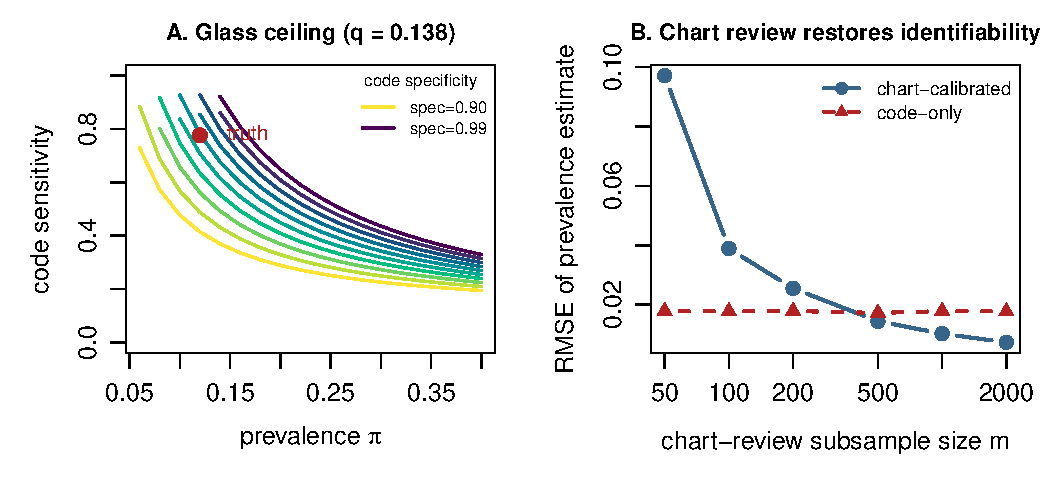
\includegraphics[width=0.95\linewidth]{glass_ceiling.pdf}
\caption{(A) Glass-ceiling solution surface. Each curve fixes a code
specificity; every point reproduces the observed code frequency $\bar
C = 0.138$ exactly. The true parameters (red) are one point among a
continuum, with implied prevalence spanning $0.06$ to $0.40$. (B)
Chart review restores identifiability: RMSE of the
chart-review-calibrated prevalence estimate falls as the reviewed
subsample size $m$ grows, while the code-only estimator's error is
flat (it is bias, not sampling error).}
\label{fig:glass}
\end{figure}

\subsection{Identifiability with chart review (\cref{thm:identifiability-chart})}

We test whether a representative chart-reviewed subsample recovers
prevalence. For $\pi = 0.12$, $b_1 = 1$, and $n = 20{,}000$, we draw a
simple random subsample of size $m$, adjudicate the true state, fit the
coding model on the subsample, and deconvolve cohort prevalence. Over
$200$ replicates per subsample size, the calibrated estimator's RMSE
decreases monotonically with $m$: $0.097$ at $m = 50$, $0.039$ at $m =
100$, $0.025$ at $m = 200$, $0.014$ at $m = 500$, $0.0102$ at $m =
1{,}000$, and $0.0073$ at $m = 2{,}000$ (\Cref{tab:chart},
\Cref{fig:glass}B). The calibrated estimator's bias is small at every
$m$ (magnitude below $0.013$ at $m = 50$ and below $0.001$ from $m =
1{,}000$ on); the RMSE at small $m$ is dominated by the variance of
fitting the coding model on few adjudicated cases.

The code-only estimator, by contrast, has RMSE essentially constant
near $0.0177$ across all $m$, because its error is bias, not sampling
noise: it estimates the code frequency, not the prevalence, and chart
review of patients it never uses cannot help it.
\Cref{thm:identifiability-chart} is confirmed: a chart-reviewed
subsample covering both classes identifies the coding model, and cohort
prevalence becomes identifiable, with estimation error shrinking at the
usual $m^{-1/2}$ rate.

\begin{table}[ht]
\centering
\begin{tabular}{rrrrr}
\toprule
$m$ & calibrated RMSE & calibrated bias & code-only RMSE & code-only bias \\
\midrule
$50$    & $0.0971$ & $+0.0129$  & $0.0178$ & $+0.0177$ \\
$100$   & $0.0389$ & $-0.0002$  & $0.0178$ & $+0.0176$ \\
$200$   & $0.0255$ & $+0.0036$  & $0.0179$ & $+0.0177$ \\
$500$   & $0.0144$ & $+0.0013$  & $0.0172$ & $+0.0171$ \\
$1{,}000$ & $0.0102$ & $+0.0010$ & $0.0178$ & $+0.0177$ \\
$2{,}000$ & $0.0073$ & $-0.0000$ & $0.0177$ & $+0.0175$ \\
\bottomrule
\end{tabular}
\caption{Chart-review-calibrated versus code-only prevalence
estimation, $\pi = 0.12$, $200$ replicates per row. The calibrated
RMSE shrinks with the reviewed subsample size $m$; the code-only error
is a fixed bias.}
\label{tab:chart}
\end{table}

\subsection{Code-frequency consistency (\cref{thm:code-total})}

The theorem predicts that a fitted phenotype model reproduces the
empirical code frequency exactly. Over $200$ replicates with $n =
20{,}000$ and a chart-review subsample of $m = 1{,}000$, the
calibrated triple $(\hat\pi, \widehat{\mathrm{sens}},
\widehat{\mathrm{spec}})$ has code-frequency residual $|\,\hat q -
\bar C\,|$ with median $0$ and maximum $3 \times 10^{-17}$, machine
precision.

The sharper check is the one \cref{thm:code-total} warns about. We take
a model with a \emph{deliberately wrong} prevalence (twice the truth)
and re-solve its sensitivity to match the observed code frequency. This
wrong-prevalence model reproduces $\bar C$ exactly: median and maximum
residual both $0$. A marginal-fit check, comparing predicted to
observed coding rate, cannot tell the wrong-prevalence model from the
correct one. The diagnostic practitioners reach for is uninformative
about the quantity of interest, exactly as the theorem states.

\subsection{Bias under informative coding (\cref{thm:bias-informative})}

\paragraph{The coding slope sweep.} We sweep the coding-mechanism
severity slope $b_1 \in \{0, 0.5, 1, 1.5, 2, 3\}$, $\pi = 0.12$, $200$
replicates per value. At $b_1 = 0$ the coding mechanism does not depend
on severity, C2 holds, and the severity-coding correlation $\rho$ is
$0$; as $b_1$ grows the marginal code sensitivity rises (from $0.50$ at
$b_1 = 0$ to $0.90$ at $b_1 = 3$) because severe cases are
preferentially coded (\Cref{tab:informative}).

The code-only estimator's bias tracks the C2 violation. At $b_1 = 0$
the bias is $-0.016$: with sensitivity only $0.50$, half of true cases
are missed, and the miss deficit $\pi(1 - \mathrm{sens})$ slightly
outweighs the false-positive inflation $(1-\pi)\,\mathrm{fpr}$, so
code-only prevalence \emph{understates} the truth. As $b_1$ rises the
sensitivity deficit shrinks faster than the false-positive inflation,
and the code-only bias swings positive: $+0.004$ at $b_1 = 0.5$,
$+0.017$ at $b_1 = 1$, $+0.025$ at $b_1 = 1.5$, $+0.028$ at $b_1 = 2$,
and $+0.032$ at $b_1 = 3$. The magnitude of the bias is governed by the
coding mechanism, not by the cohort size, exactly as
\cref{thm:bias-informative} predicts. The chart-review-calibrated
estimator stays near-unbiased throughout: its bias magnitude is below
$0.002$ at every $b_1$, and its RMSE falls from $0.019$ at $b_1 = 0$ to
$0.0084$ at $b_1 = 3$ (\Cref{fig:informative}A).

\begin{table}[ht]
\centering
\begin{tabular}{rrrrr}
\toprule
$b_1$ & $\rho$ & code-only bias & calibrated bias & MCSE \\
\midrule
$0.0$ & $0.000$ & $-0.0161$ & $+0.0030$ & $0.0013$ \\
$0.5$ & $0.994$ & $+0.0045$ & $+0.0008$ & $0.0009$ \\
$1.0$ & $0.954$ & $+0.0174$ & $+0.0010$ & $0.0008$ \\
$1.5$ & $0.894$ & $+0.0247$ & $+0.0015$ & $0.0007$ \\
$2.0$ & $0.834$ & $+0.0286$ & $-0.0002$ & $0.0006$ \\
$3.0$ & $0.743$ & $+0.0322$ & $+0.0001$ & $0.0006$ \\
\bottomrule
\end{tabular}
\caption{Bias under informative coding, $\pi = 0.12$, $200$ replicates
per row. The coding slope $b_1$ controls the C2 violation; $b_1 = 0$ is
non-informative coding. $\rho$ is the severity-coding correlation among
true cases, and is \emph{non-monotone} in $b_1$ (it rises to $0.994$ at
$b_1 = 0.5$ then falls to $0.743$ at $b_1 = 3.0$), so violation
severity is indexed by $|b_1|$, not $\rho$. The calibrated column uses
the \emph{deployable} weighted-by-$\widehat\Prob(\Y\mid S)$ estimator
(\cref{sec:methodology}; no latent cohort labels), with the same
representative review used throughout. MCSE is the Monte Carlo
standard error (sample standard deviation across replicates divided by
$\sqrt{200}$). The code-only bias is driven by the coding mechanism and
is many MCSEs from zero at every $b_1$; the deployable calibrated
estimator's bias sits within roughly two MCSEs of zero throughout,
statistically indistinguishable from unbiased. The oracle reference
(averaging over $\{S : \Y = 1\}$ in the full cohort) gives calibrated
bias within $0.003$ of the deployable column at every $b_1$, so the
remedy does not depend on knowing the latent labels.}
\label{tab:informative}
\end{table}

The correlation $\rho$ is near $1$ for small $b_1$ and declines as
$b_1$ grows, because a steep logistic in severity saturates and becomes
nonlinear, loosening the linear association between $S$ and the code
probability. The informative-coding contribution to the bias is
nonetheless real at every $b_1 > 0$: the bound \eqref{eq:meth-bound}
controls the gap between the marginal cohort sensitivity and the
average-severity coding probability by $|b_1|\,\sigma_{S,1}/4$, and the
swing in marginal sensitivity as $b_1$ grows is what drives the swing
in code-only bias.

\paragraph{The case-mix gap.} \Cref{cor:casemix} predicts that when the
chart-reviewed subsample is not representative of the cohort, the
calibrated estimator inherits a residual bias proportional to the
case-mix sensitivity gap. We test this by drawing a severity-biased
chart-review subsample: a patient's probability of being selected for
review rises with severity, controlled by a selection slope. As the
selection slope grows from $0$ to $2$, the sensitivity gap between the
reviewed subsample and the cohort grows from $0.001$ to $0.036$
(\Cref{tab:casemix}).

A calibrated estimator that marginalizes code sensitivity over the
reviewed subsample's own severity distribution inherits this gap: its
residual bias grows in magnitude from $-0.0007$ at gap $0.001$ to
$-0.006$ at gap $0.036$. A calibrated estimator that marginalizes over
the cohort severity distribution does not: its bias stays within
$\pm 0.001$ of zero throughout (\Cref{fig:informative}B). The
sensitivity gap saturates near $0.036$ for selection slopes from $1.0$
to $2.0$ because the per-case code probability $\mathrm{logit}^{-1}(b_0
+ b_1 S)$ is itself bounded above by $1$: once severity-biased
selection concentrates the reviewed subsample at the top of the
severity distribution, the subsample-marginal sensitivity approaches
the logistic ceiling and the gap stops growing. The marginal
sensitivity over true cases itself rises from $0.500$ at $b_1 = 0$
toward (but not reaching) $0.902$ at $b_1 = 3$, the same logistic
saturation. This is the phenotyping analog of the ERCC-endogenous
capture-efficiency gap of \citet{towell2026scrnacoarsening}:
chart-reviewed patients restore identifiability only to the extent
that they are drawn from the same population as the cohort being
corrected.

\begin{table}[ht]
\centering
\begin{tabular}{rrrr}
\toprule
review selection slope & sensitivity gap & subsample-ref bias & cohort-ref bias \\
\midrule
$0.0$ & $0.001$ & $-0.0007$ & $-0.0005$ \\
$0.5$ & $0.026$ & $-0.0039$ & $+0.0003$ \\
$1.0$ & $0.034$ & $-0.0046$ & $+0.0005$ \\
$1.5$ & $0.037$ & $-0.0064$ & $-0.0008$ \\
$2.0$ & $0.036$ & $-0.0060$ & $-0.0003$ \\
\bottomrule
\end{tabular}
\caption{Residual bias of the chart-review-calibrated estimator under
a severity-biased review subsample, $\pi = 0.12$, $200$ replicates per
row. The subsample-reference estimator inherits the case-mix gap; the
cohort-reference estimator does not.}
\label{tab:casemix}
\end{table}

\begin{figure}[t]
\centering
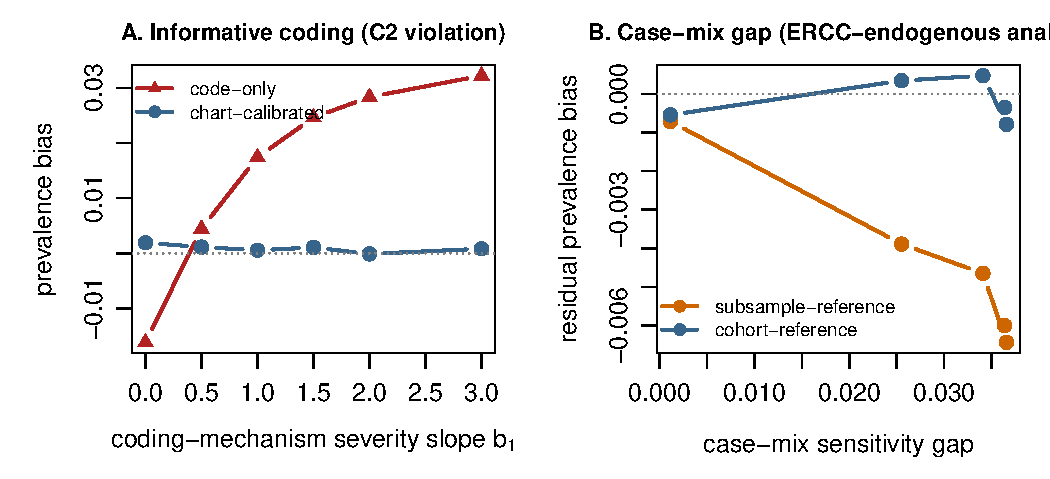
\includegraphics[width=0.95\linewidth]{informative_coding.pdf}
\caption{(A) Prevalence bias as the coding-mechanism severity slope
$b_1$ grows (the C2 violation strengthens). The code-only estimator's
bias is governed by the coding mechanism; the chart-review-calibrated
estimator stays near zero. (B) Residual bias of the calibrated
estimator as the case-mix sensitivity gap grows. Using the cohort
severity distribution as the reference removes the residual bias;
using the reviewed subsample's own distribution inherits it.}
\label{fig:informative}
\end{figure}

\subsection{Real-data plan: MIMIC-IV}

The natural real-data anchor is MIMIC-IV \citep{johnson2023mimiciv}, a
publicly available critical-care EHR dataset containing ICD diagnosis
codes, procedures, and medication orders alongside rich clinical data
(laboratory results, vital signs, clinician notes). The clinical data
can serve as a chart-review proxy: a structured rule over labs and
physiology, or a manual review of notes, supplies an adjudicated state
$\Y$ that plays the role of the chart-reviewed singleton candidate set,
while the ICD code plays the role of the coarse observation $C$.

The planned analysis takes a condition with a recognized
code-versus-chart discrepancy (for example, acute kidney injury, where
the diagnosis code is known to undercount laboratory-defined cases) and
(i) estimates code-only prevalence from the ICD code, (ii) estimates
the chart-proxy prevalence from the laboratory definition, (iii) fits
the coding model and the severity dependence on the chart-proxy
subsample, (iv) deconvolves cohort prevalence via \eqref{eq:deconvolve},
and (v) checks code-frequency consistency (\cref{thm:code-total})
directly on the cohort. For AKI we preregister the chart-proxy as
KDIGO stage 1 or higher \citep{kdigo2012aki}: a serum creatinine
increase of at least $0.3$ mg/dL within $48$ hours, an increase to at
least $1.5\times$ baseline within $7$ days, or urine output below $0.5$
mL/kg/h sustained for at least $6$ hours. A stratified chart-proxy subsample, balanced
across encounter intensity and code status, lets the case-mix gap
$\delta$ of \cref{cor:casemix} be estimated and reported. This
real-data application is described here and left as the principal
pending item; the simulation is the core validation for the present
version.

\section{Discussion}
\label{sec:discussion}

\subsection{Relation to prior work}

The estimation problem this paper addresses, recovering disease
prevalence and code error rates without a perfect reference, has a
substantial prior literature, and we want to be precise about what is
and is not new.

\paragraph{Prevalence correction and latent-class diagnostic-test
models.} The deconvolution \eqref{eq:deconvolve} that supplies the
chart-review-calibrated prevalence estimator is the
\citet{rogan1978estimating} formula, a textbook screening-test
correction: given known sensitivity and specificity, apparent
prevalence is inverted to true prevalence. Rogan and Gladen presume
the two error rates known precisely because, as \cref{thm:glass-ceiling}
makes explicit, the triple $(\pi, \mathrm{sens}, \mathrm{spec})$ is
non-identifiable from code data alone. \citet{hui1980estimating} is
the foundational latent-class work: it estimates the sensitivity and
specificity of diagnostic tests, and the prevalence of disease, by
treating the true disease status as a latent class and fitting
multiple imperfect tests jointly. The estimator of
\cref{thm:identifiability-chart} is, in the case of two coarse features
and no chart review, a Hui-Walter latent-class model. We do not claim
to originate latent-class estimation of disease status, nor the
estimation of sensitivity and specificity without a gold standard, nor
the Rogan-Gladen plug-in. \citet{dawid1979maximum} is the
methodological ancestor one step further back: the EM algorithm for
observer (rater) error rates, which is the same latent-variable
maximum-likelihood computation applied to disagreeing raters rather
than disagreeing tests. The coding mechanism of \cref{sec:translation}
is a rater-error model in which the rater is the EHR coding process.

\paragraph{Verification bias.} The case-mix-gap residual bound
(\cref{cor:casemix}) belongs substantively to the verification-bias
literature in diagnostic-test evaluation. \citet{begg1983assessment}
showed that when verification of disease status is selective (so the
chart-reviewed or biopsy-confirmed subsample is not a random sample of
those screened), apparent sensitivity and specificity are biased, and
the bias propagates into prevalence and predictive-value estimates;
this is the now-standard verification-bias correction
\citep{hubbard2020outcome}. The substantive content of
\cref{cor:casemix} is a verification-bias statement: the subsample
sensitivity is not transportable to the cohort when chart review is
selective. What the coarsening framing contributes is positioning:
verification bias becomes a C2 failure on the chart-reviewed subsample
(non-informative coding fails within the reviewed group as it does
within the cohort), and the singleton candidate sets supplied by chart
review identify the cohort coding model only insofar as the reviewed
case mix matches. The contribution of this paper is the recasting and
the unification, not the verification-bias result itself.

\paragraph{Electronic phenotyping efforts.} eMERGE
\citep{gottesman2013emerge,newton2013validation} and the PheKB catalog
\citep{kirby2016phekb} are large phenotyping programs that build and
share code-based phenotype algorithms. PheWAS \citep{denny2010phewas}
treats code groupings as phenotypes directly.
\citet{banda2018phenotyping} surveys the methodological landscape from
rule-based to machine-learning phenotyping; \citet{liao2015highthroughput}
develop high-throughput algorithms with NLP; PheNorm
\citep{yu2018phenorm} and PheCAP \citep{zhang2019phecap} are
semi-supervised methods that reduce the labeling burden;
\citet{pivovarov2015learning} fits probabilistic phenotypes
end-to-end. The anchor-and-learn framework \citep{halpern2016anchor}
learns phenotype classifiers using high-precision ``anchor''
observations whose presence almost certainly implies the true state;
an anchor is structurally a near-singleton candidate set, and
\citet{halpern2016anchor} is the closest prior work in spirit to the
singleton-restores-identifiability mechanism of this paper.
Surveillance bias, the phenomenon that more intense looking finds more
disease, is named by \citet{haut2011surveillance} and quantified as a
phenotyping artifact by \citet{carrell2014surveillance}. The
EHR-as-data perspective of \citet{hripcsak2013correlating} and the
OHDSI treatment-pathway work of \citet{hripcsak2016characterizing}
frame the data-quality and process-dependence issues that the
coarsening lens makes precise.

\paragraph{What is new here.} The contribution is not latent-class
phenotyping. It is the masked-cause unification: (i) the explicit
candidate-set translation that places code-based phenotyping inside the
coarsening-at-random framework of \citet{towell2026masked}; (ii) the
C1-C2-C3 classification that identifies informative coding as
specifically a C2 violation, distinguishing it from miscoding (C1) and
from confounding between coding parameters and prevalence (C3); (iii)
the explicit glass-ceiling construction (\cref{thm:glass-ceiling}),
which exhibits the non-identifiable solution surface rather than
asserting non-identifiability; and (iv) the informative-coding bias
bound (\cref{thm:bias-informative}) and the case-mix-gap residual bound
(\cref{cor:casemix}), which quantify the bias of the code-only and
calibrated estimators in terms of interpretable quantities, the
severity-coding correlation and the case-mix gap. The Hui-Walter model
tells a practitioner \emph{that} prevalence can be estimated from
imperfect tests; the coarsening framework tells the practitioner
\emph{which assumption} (C2) the EHR violates, \emph{why} (informative
coding), and \emph{how large} the resulting bias is.

\subsection{What the framework does not address}

\begin{itemize}
\item \textbf{Multi-code phenotypes and temporal structure.} We treat
  the candidate set as generated by a small set of binary codes
  observed cross-sectionally. Real phenotype algorithms use code counts,
  code timing, medication sequences, and laboratory trajectories. The
  framework extends to richer candidate sets, but the present analysis
  does not.

\item \textbf{Chart review error.} We treat the chart-reviewed state as
  a true singleton. Adjudication itself is imperfect, and inter-rater
  disagreement is exactly the setting of \citet{dawid1979maximum}. The
  framework would benefit from incorporating chart-review error via the
  C2-relaxation results of \citet{towell2026mdrelax}.

\item \textbf{The form of the coding mechanism.} The bias bound
  \eqref{eq:meth-bound} assumes a logistic coding mechanism with a
  scalar severity. Real coding depends on insurance, site, clinician,
  and calendar time. A more flexible misspecification model is needed.

\item \textbf{Causal estimands.} We target descriptive cohort
  prevalence. Phenotyping feeds downstream association and
  causal-inference analyses, where informative coding induces further
  bias (differential misclassification of the exposure or outcome). The
  propagation of the coarsening bias into those estimands is left open.

\item \textbf{Identifiability from codes alone via parametric
  restriction.} \Cref{thm:glass-ceiling} concerns an unrestricted
  coding mechanism. With a sufficiently restricted parametric family,
  or multiple conditionally independent codes as in
  \citet{hui1980estimating}, prevalence can be identified without chart
  review. Characterizing exactly which restrictions suffice, and how
  fragile the resulting estimates are, is a natural follow-up.
\end{itemize}

\subsection{Sibling applications of the framework}

The masked-data lens has now been applied across a small set of
measurement domains.
In single-cell RNA sequencing, \citet{towell2026scrnacoarsening} treats
dropout zeros as candidate-set ambiguity and identifies ERCC
spike-ins as the singleton mechanism. In spatial transcriptomics,
\citet{towell2026spatialcoarsening} ports the rank condition to
cell-type deconvolution within spots. In differential privacy,
\citet{towell2026dpcoarsening} treats noisy release as the masking
mechanism and characterizes identifiability of population parameters
under privacy budgets. In programmatic weak supervision,
\citet{towell2026weaksupcoarsening} treats labeling functions as
candidate sets and develops identifiability conditions in the absence
of a gold standard. Electronic phenotyping joins this family as the
healthcare-data instance: the same masked-cause structure with the
same singleton-restores-identifiability mechanism, distinguished by
informative coding as the dominant C2 violation rather than (as in
the transcriptomics applications) a comparatively mild deviation from
non-informative observation. Recognition of this common structure may
streamline methodology across these subfields.

\section{Conclusion}
\label{sec:conclusion}

Code-based phenotyping has been refined methodologically through
latent-class fits, anchor learning, semi-supervised algorithms, and
high-throughput pipelines, yet the structural reason its prevalence
estimates are biased has stayed informal. The masked-data framing
gives the structure a name. Informative coding is a C2 violation;
chart review is a singleton candidate set; the Rogan-Gladen plug-in is
the deconvolution it enables; marginal-fit blindness is the
identifiability cost of working with only the cohort code frequency;
the case-mix gap is the limit on what review can recover.

This recasting moves the practitioner's question from method-specific
(``should I use PheCAP or PheNorm?'') to assumption-specific (``does
my coding mechanism violate C2, and is my chart-reviewed subsample
representative of the cohort?''). The diagnosis is almost always that
C2 fails. The framework then says precisely what is required: singleton
candidate sets, supplied by chart review, anchor observations, or a
gold-standard registry, sampled to match the cohort case mix; a
reported case-mix gap as a sensitivity quantity; and recognition that
the marginal-fit check is silent on prevalence error.

The same coarsening structure appears across health-data measurement
problems with the same informative-observation issue: claims-based
comorbidity indices, registry case-finding, cause-of-death coding, and
adverse-event surveillance. In each case a latent clinical truth is
observed only through an administrative process whose intensity depends
on the truth, and the C1-C2-C3 conditions and the identifiability
machinery transfer directly.

Three extensions sit naturally next. First, multi-code and temporal
candidate sets: real phenotype algorithms aggregate code counts, code
timing, medication sequences, and lab trajectories, and the
identifiability rank conditions extend but have not been worked out.
Second, chart-review error: adjudication is itself imperfect, and the
C2-relaxation results of \citet{towell2026mdrelax} would let the
singleton assumption itself be relaxed. Third, propagation: code-based
phenotypes feed downstream association and causal-inference analyses,
where informative coding induces differential misclassification of the
exposure or outcome, and the propagation of the coarsening bias into
those estimands is open.

The contribution this paper makes is positioning. It places electronic
phenotyping inside a unified vocabulary that names the failing
assumption (C2), supplies the remedy (singleton candidate sets), and
quantifies the residual (the case-mix gap). The technical results are
not breakthroughs in isolation, they are corollaries of the
masked-data framework applied to the specific structure of EHR coding,
but the unification is what lets a clinician or methodologist read off,
from the coding mechanism and the chart-review sampling, the direction
and bounded magnitude of the prevalence error they will incur.


\bibliographystyle{plainnat}
\bibliography{refs}

\end{document}
